\subsection{Wägezelle}

Wägezellen messen mechanische Verformungen.
Wird auf eine Wägezelle eine Gewichtskraft \mbox{$F = m \cdot g \: [\frac{kg \cdot m}{s^2}]$} (m = aufgebrachte Masse und $g = 9.81 \: \frac{m}{s^2}$)  aufgebracht, verformt sich diese unter der Krafteinwirkung.
Auf der Wägezelle sind Dehnungsmessstreifen aufgebracht, deren Widerstand sich bei Verformung ändert.
Die Dehnungsmessstreifen sind in einer Wheatstone-Brücke verschaltet, die die Widerstandsänderung in eine Spannungsänderung umwandelt, die meist nur im Bereich weniger Millivolt liegt.
Diese Spannungsänderung ist proportional zur aufgebrachten Gewichtskraft. Unten dargestellt in \autoref{CAD Darstellung Wägezelle} ist der Aufbau einer Wägezelle als CAD-Modell. \\
\begin{figure}
    \centering
    \includegraphics[width=0.9\textwidth]{img/CAD Wägezelle.png}
    \captionof{figure}{CAD Darstellung Wägezelle}\label{CAD Darstellung Wägezelle}
\end{center}

\subsection{Elektromyographie}

Mit einem EMG kann die elektrische Muskel-Aktivität gemessen werden.

Dazu wird die elektrische Aktivität in einem ruhenden und einem kontrahierten Muskel gemessen. Das Signal entsteht aus dem Aktionspotential der Muskelfasermembran und dem Depolarisations- und Repolarisationsverlauf, der in \autoref{Depolarisations- und Repolarisationsverlauf} als Funktion der Zeit dargestellt ist. Im Ruhetonus liegt das Potential zwischen $-80$ und  $-90$ mV.

\begin{center}[h!]
    \centering
    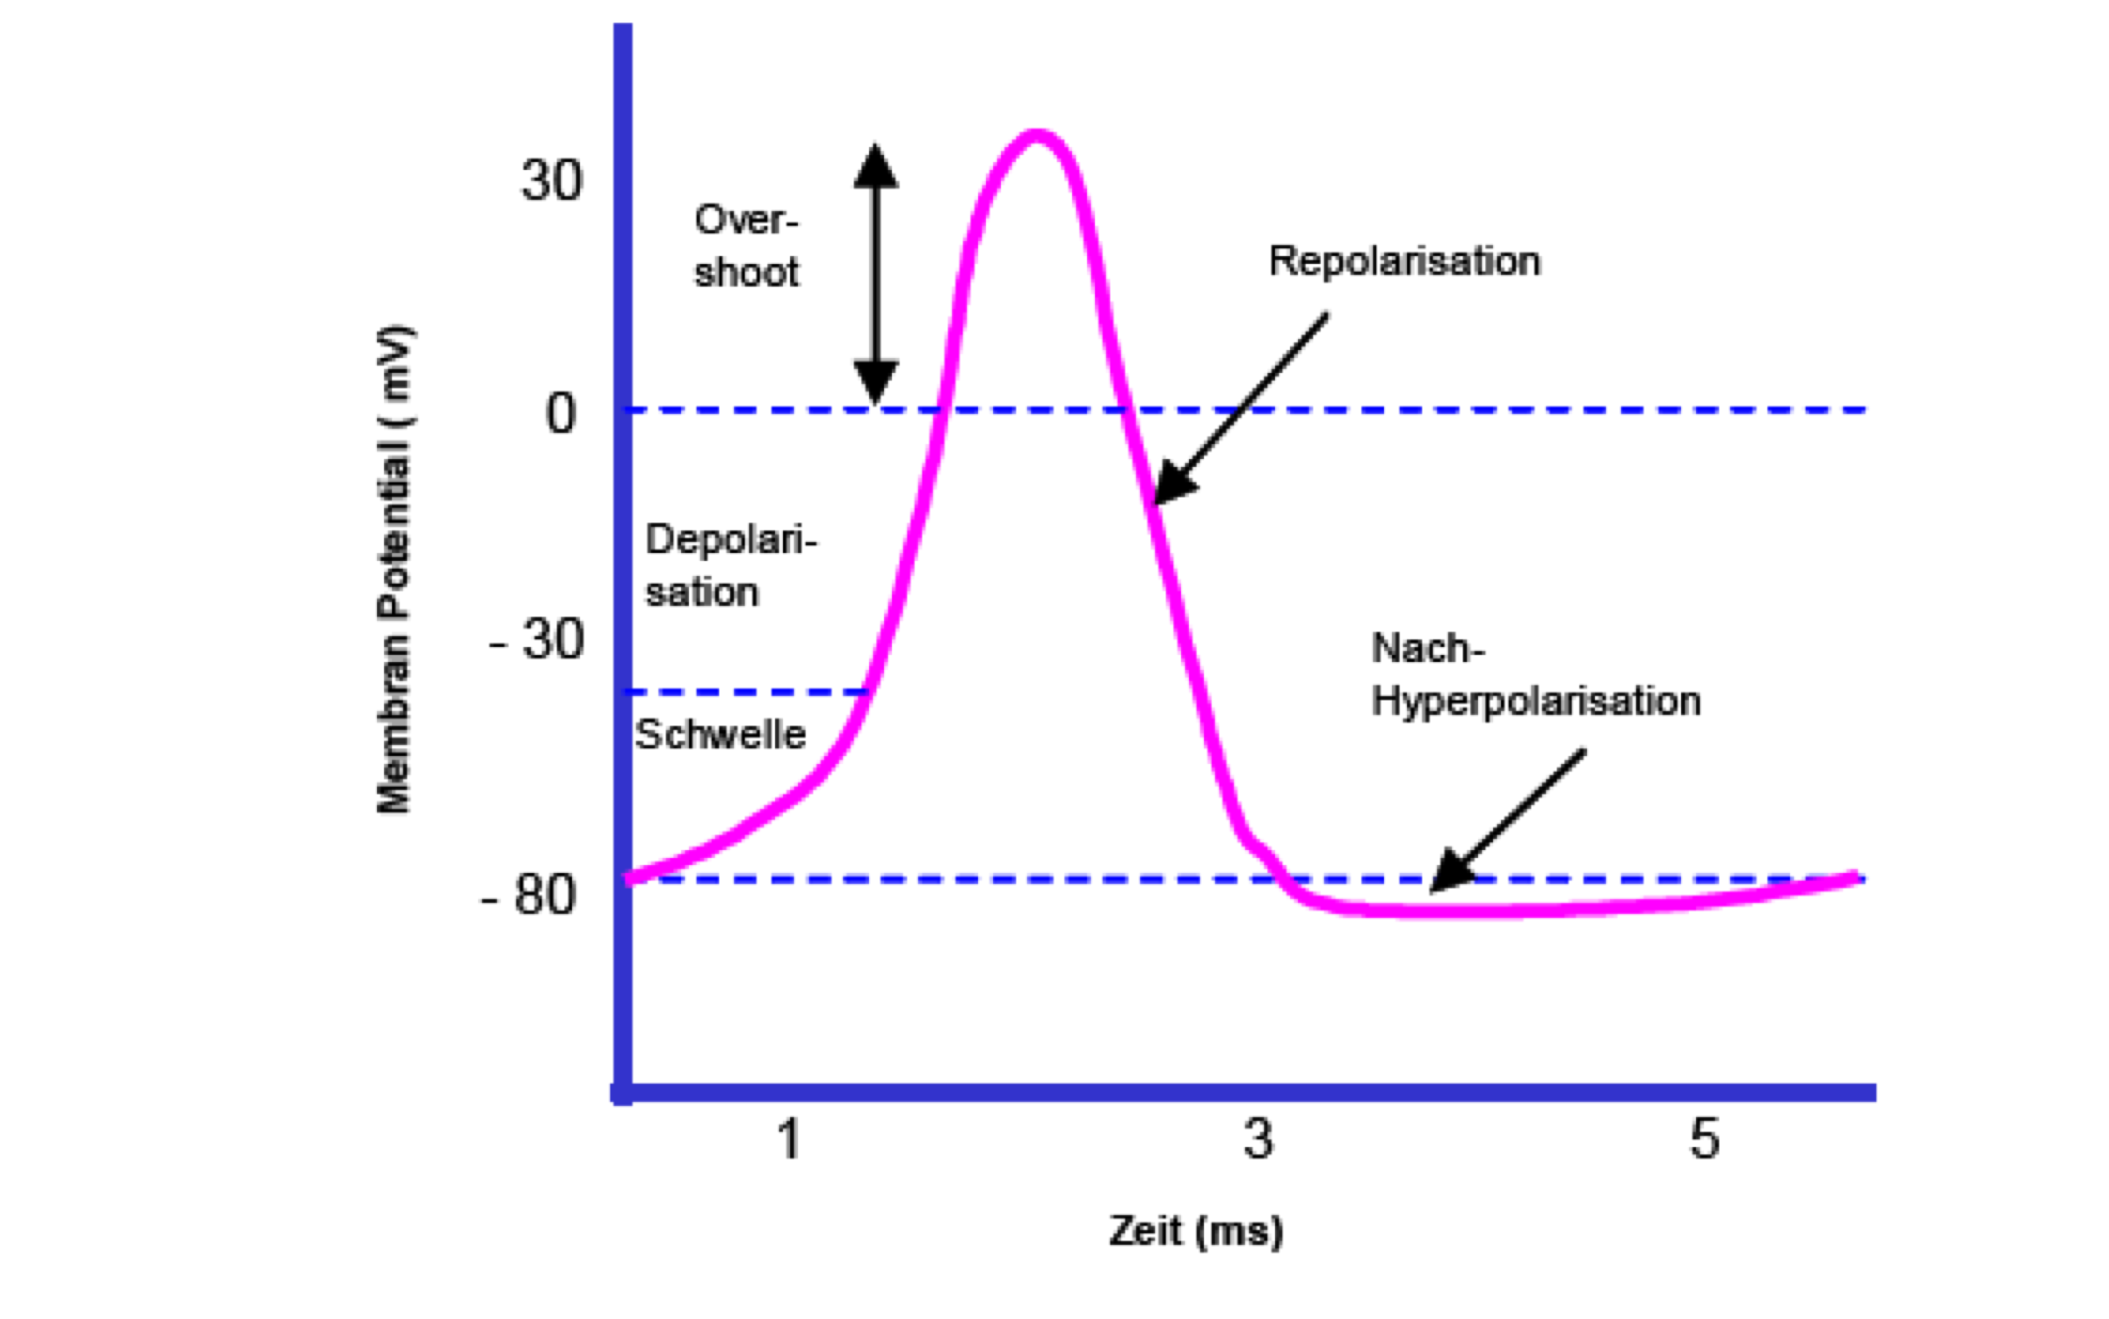
\includegraphics[width=0.8\textwidth]{img/De- Repolarisation.PNG}
    \captionof{figure}[De- und Repolarisation und Aktionspotential Muskelfasermembran]{De- und Repolarisation und Aktionspotential Muskelfasermembran \cite{Vorlesung-Muskulatur-EMG}}\label{Depolarisations- und Repolarisationsverlauf}
\end{center}

Eine Muskelkontraktion startet auf Sarkomerebene. Durch das Zusammenwirken aller Sarkomere wird die Umwandlung von chemischer Energie in mechanische Energie als Kontraktion des Muskels sichtbar.\\
\\
Ein  Nervenimpuls gelangt als Aktionspotential über das Axon eines Motoneurons zum Axonende. \\
Durch Neurotransmitter die in den postsynaptischen Spalt ausgeschüttet und dann an den Rezeptor der postsynaptischen Membran binden, wird der Prozess der Depolarisation in der Muskelfaser ausgelöst, der auf der linken Seite von  \autoref{Depolarisations- und Repolarisationsverlauf} dargestellt ist:\\
\\
Der Rezeptor ist ein Kanal für Kationen, also positiv geladene Ionen wie Natrium-, Calcium- oder Kaliumionen. Wird der Ionenkanal geöffnet, kommt es zum Einfluss von Kationen und zu einer  Depolarisation der Muskelfaser. Wird ein gewisses Schwellenpotential überschritten, öffnen sich spannungsabhängige Natrium-Kanäle, wodurch ein Aktionspotential ausgelöst wird, das als EMG-Signal gemessen werden kann. In \autoref{Depolarisations- und Repolarisationsverlauf} als Schwelle gekennzeichet, ab der die Steigung der Potential-Funktion zunimmt, bis die Funktion bis $+20$ bis $+30$ mV steigt.
Das Aktionenpotential löst nun wiederum die Öffnung von spannungsgesteuerten Calcium-Kanälen aus, wodurch Calcium-Ionen in der Muskelfaser freigesetzt werden. Es kommt zu einer Anhäufung von Calcium-Ionen in der Muskelfaser. Dadurch steigt Calciumkonzentration, was die Kontraktion der Muskelfaser auslöst. \\
Noch bevor der Höhepunkt des Aktionspotentials erreicht ist, werden die Natriumkanäle inaktiv und positiv geladene Kalium strömen aus der Zelle. Das Potential nähert sich nach einer Hyperpolarisationsphase, während der das Pontential unter das Ruhepotential von $-80$ mV fällt, wieder dem Ruhepotential an.

Die EMG-Messung findet in der Hochschule im Labor für Ergonomie statt. Die Daten werden mithilfe eines Programms von NORAXON ausgelesen und analysiert.


